\documentclass[11pt,a4paper]{article}
\usepackage[margin=1in]{geometry}
\usepackage{booktabs}
\usepackage{hyperref}
\usepackage{xcolor}
\usepackage{graphicx}
\usepackage{subcaption}
\hypersetup{colorlinks=true, linkcolor=blue, urlcolor=blue, citecolor=blue}
\usepackage{titlesec}

% Appendix-style section numbering
\renewcommand{\thesection}{A.\arabic{section}}
\renewcommand{\thesubsection}{A.\arabic{section}.\arabic{subsection}}

\begin{document}

\begin{center}
{\Large\bfseries Appendix: Dataset Information}
\end{center}

\vspace{0.5em}

MELON is evaluated on five real-world spatial multi-omics datasets spanning different tissues, organisms, platforms, and modality combinations. Table~\ref{tab:datasets} summarizes the datasets used in our experiments.

\begin{table}[h]
\centering
\caption{Summary of datasets used in experiments.}
\label{tab:datasets}
\small
\begin{tabular}{llll}
\toprule
Dataset & Tissue & Modalities \\
\midrule
Mouse E13 Embryo    & Whole mouse embryo      & RNA + ATAC \\
Y7\_T (ccRCC Tumor) & Human kidney tumor      & RNA + SM (MALDI-MSI) \\
Mouse E15.5 Brain   & Embryonic mouse brain   & RNA + ATAC \\
Human Lymph Node    & Human lymph node        & RNA + Protein (ADT) \\
Human Hippocampus   & Adult human brain       & RNA + ATAC \\
\bottomrule
\end{tabular}
\end{table}

\section{Mouse E13 Embryo (spatial-ATAC-RNA-seq)}

This dataset profiles a whole E13 mouse embryo using spatial-ATAC-RNA-seq (Zhang et al., 2023), which co-profiles the epigenome and transcriptome via deterministic barcoding in tissue (DBiT-seq). Ground-truth annotations comprise embryonic tissue regions.

\begin{figure}[h]
\centering
\begin{subfigure}[t]{0.3\textwidth}
\centering
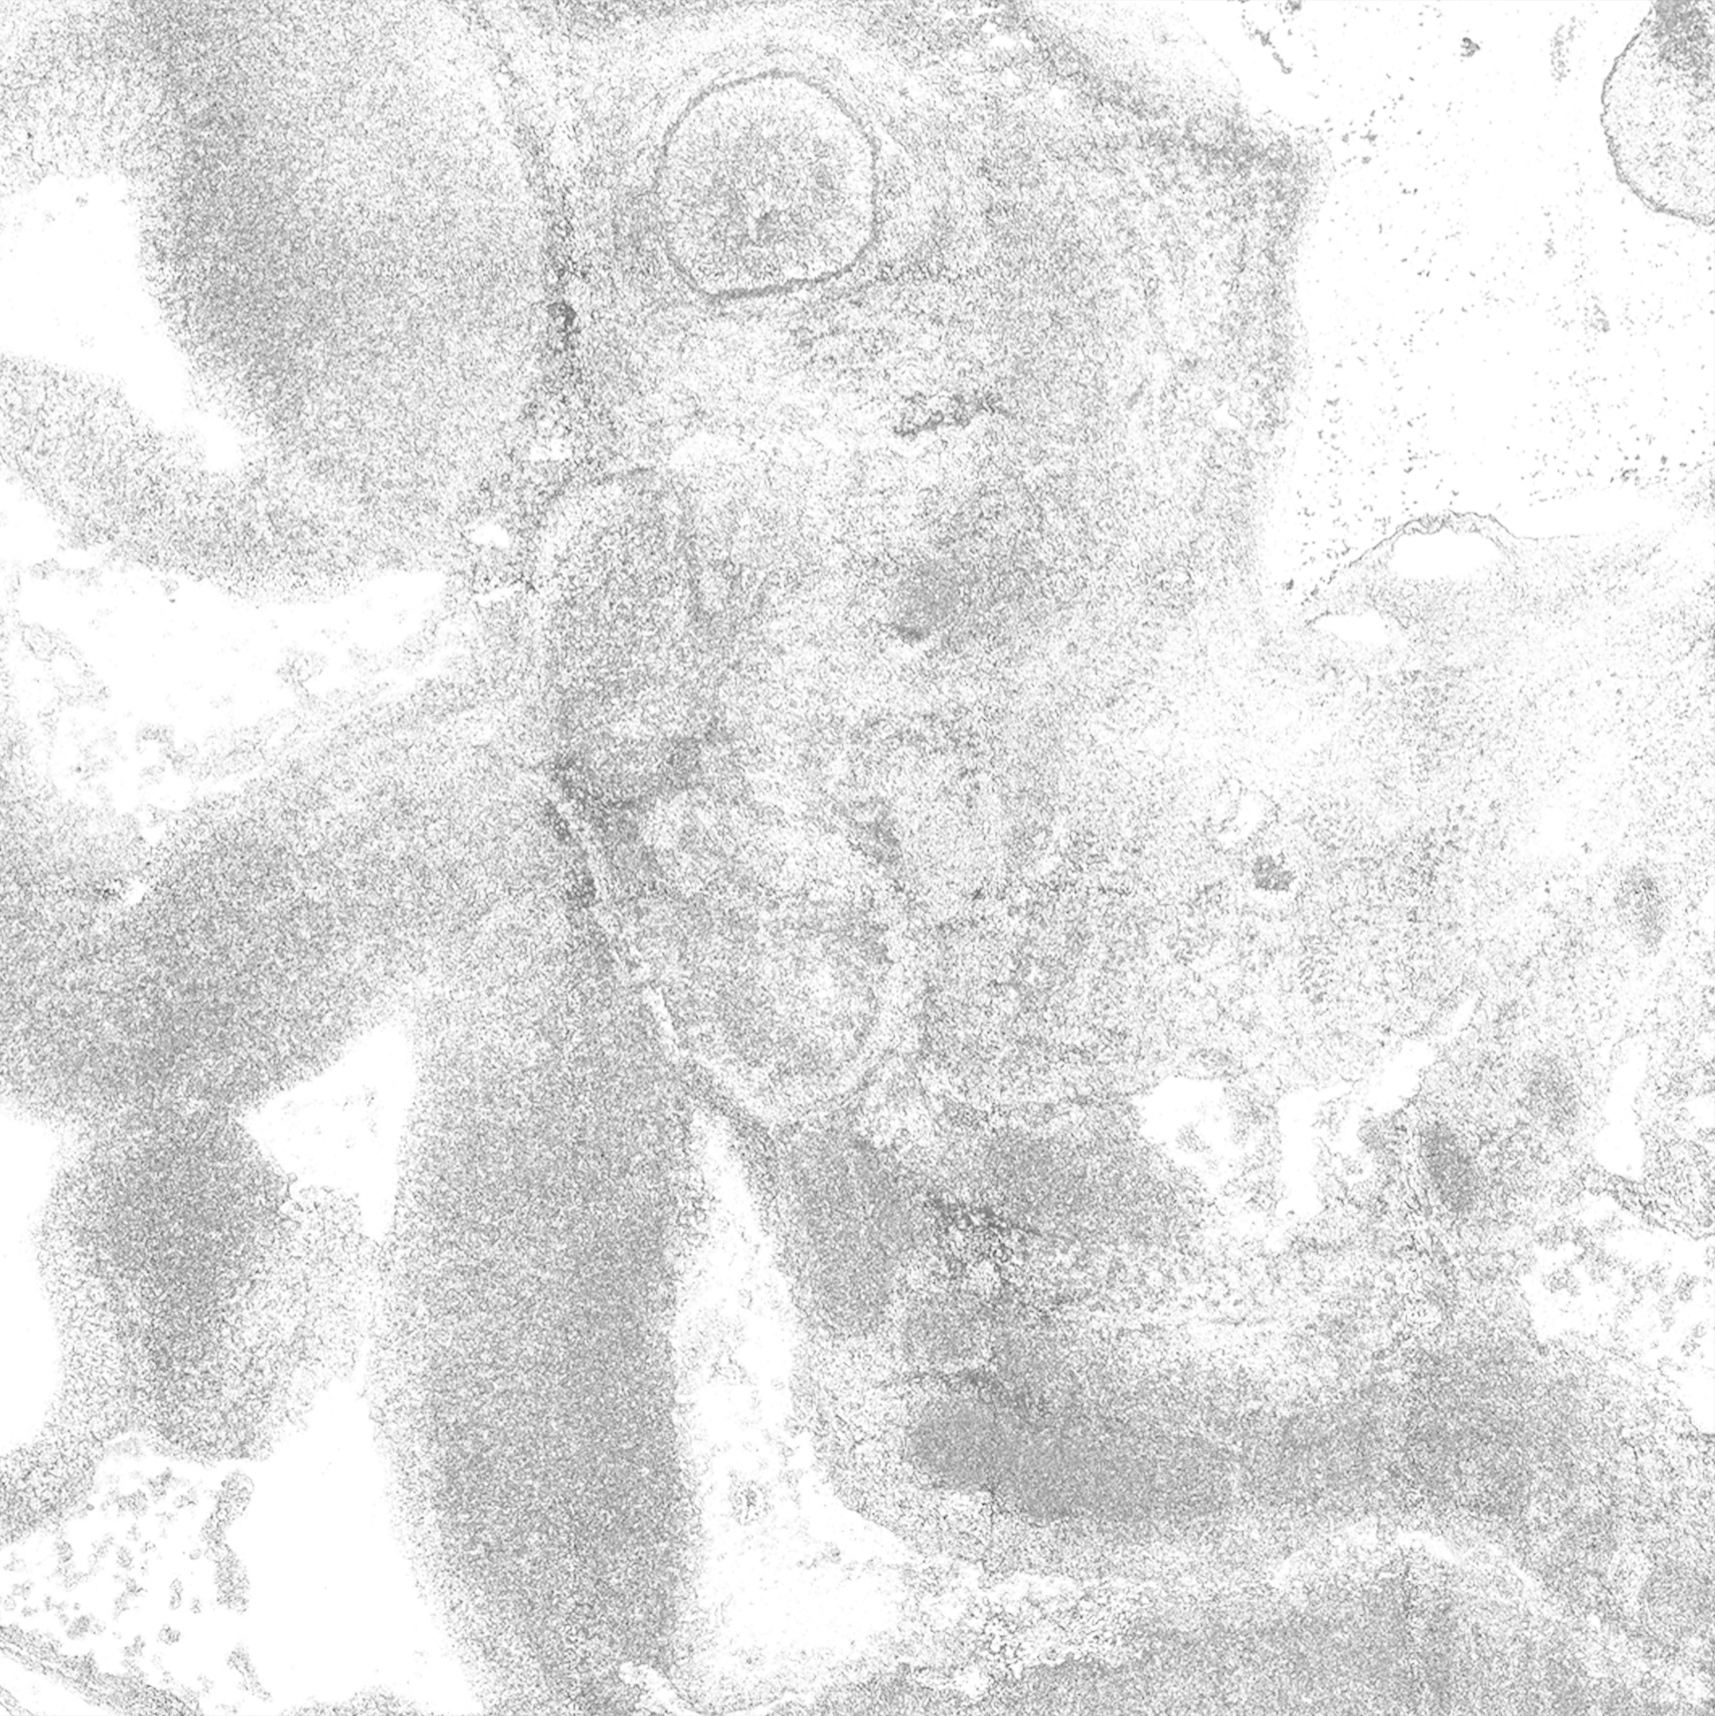
\includegraphics[width=\textwidth]{pic/he/Mouse_e13_embryo.png}
\caption{H\&E staining}
\end{subfigure}
\hfill
\begin{subfigure}[t]{0.3\textwidth}
\centering
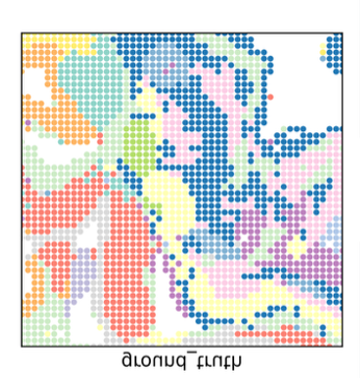
\includegraphics[width=\textwidth]{pic/anno/e13_embryo_label.png}
\caption{Ground-truth annotation}
\end{subfigure}
\hfill
\begin{subfigure}[t]{0.3\textwidth}
\centering
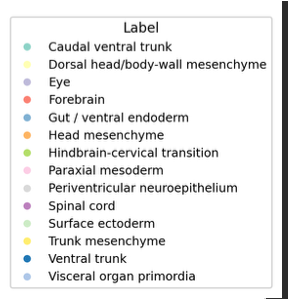
\includegraphics[width=\textwidth]{pic/anno/e13_embryo_legend.png}
\caption{Region legend}
\end{subfigure}
\caption{Mouse E13 Embryo: H\&E image and spatial domain annotations.}
\label{fig:e13}
\end{figure}

\paragraph{Reference.} Zhang, D., Deng, Y. et al. \href{https://doi.org/10.1038/s41586-023-05795-1}{Spatial epigenome--transcriptome co-profiling of mammalian tissues}. \textit{Nature}, 616(7955), 113--122, 2023.

\section{Y7\_T ccRCC Tumor Slice (Kidney)}

Y7\_T is a clear cell renal cell carcinoma (ccRCC) tumor slice from the kidney, profiled by spatial transcriptomics (RNA, gene expression) and spatial metabolomics (SM, MALDI-MSI, 1{,}299 m/z features). This dataset illustrates intra-tumoral heterogeneity, with both classical clear cell-like regions and a localized DCCD-like (distal convoluted and collecting duct-like) shift.

\begin{figure}[h]
\centering
\begin{subfigure}[t]{0.3\textwidth}
\centering
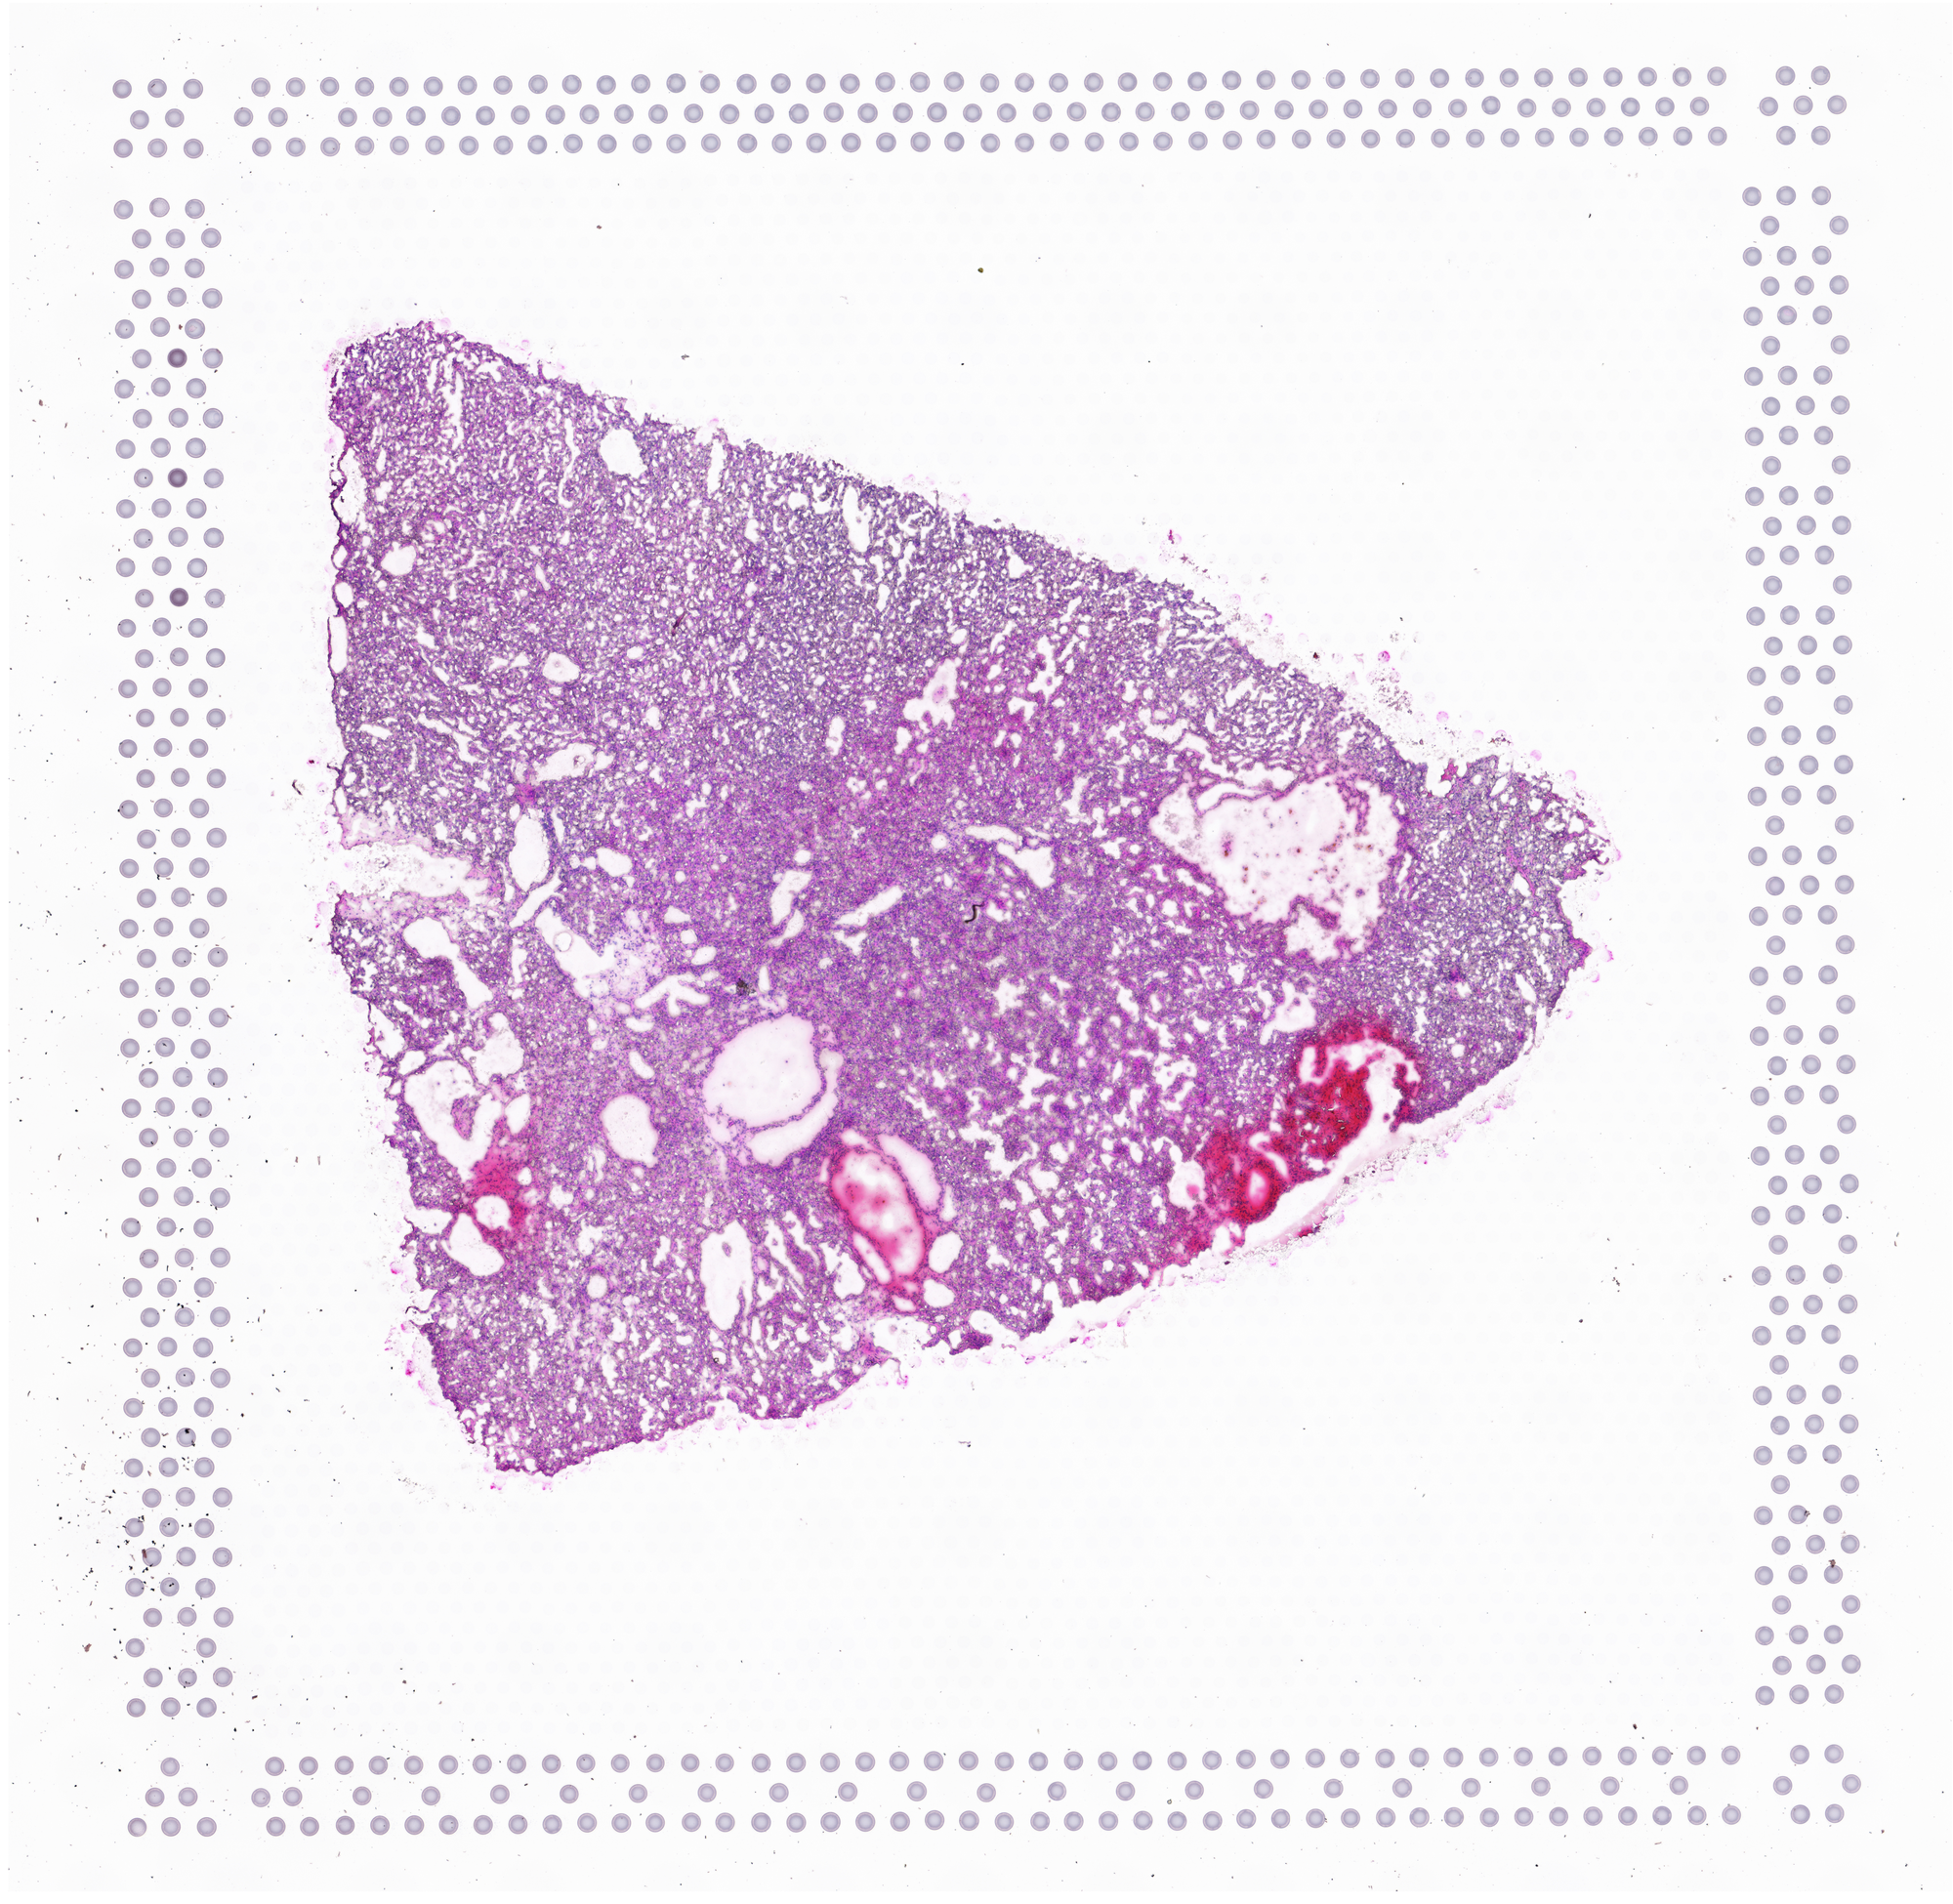
\includegraphics[width=\textwidth]{pic/he/Y7_T.png}
\caption{H\&E staining}
\end{subfigure}
\hfill
\begin{subfigure}[t]{0.3\textwidth}
\centering
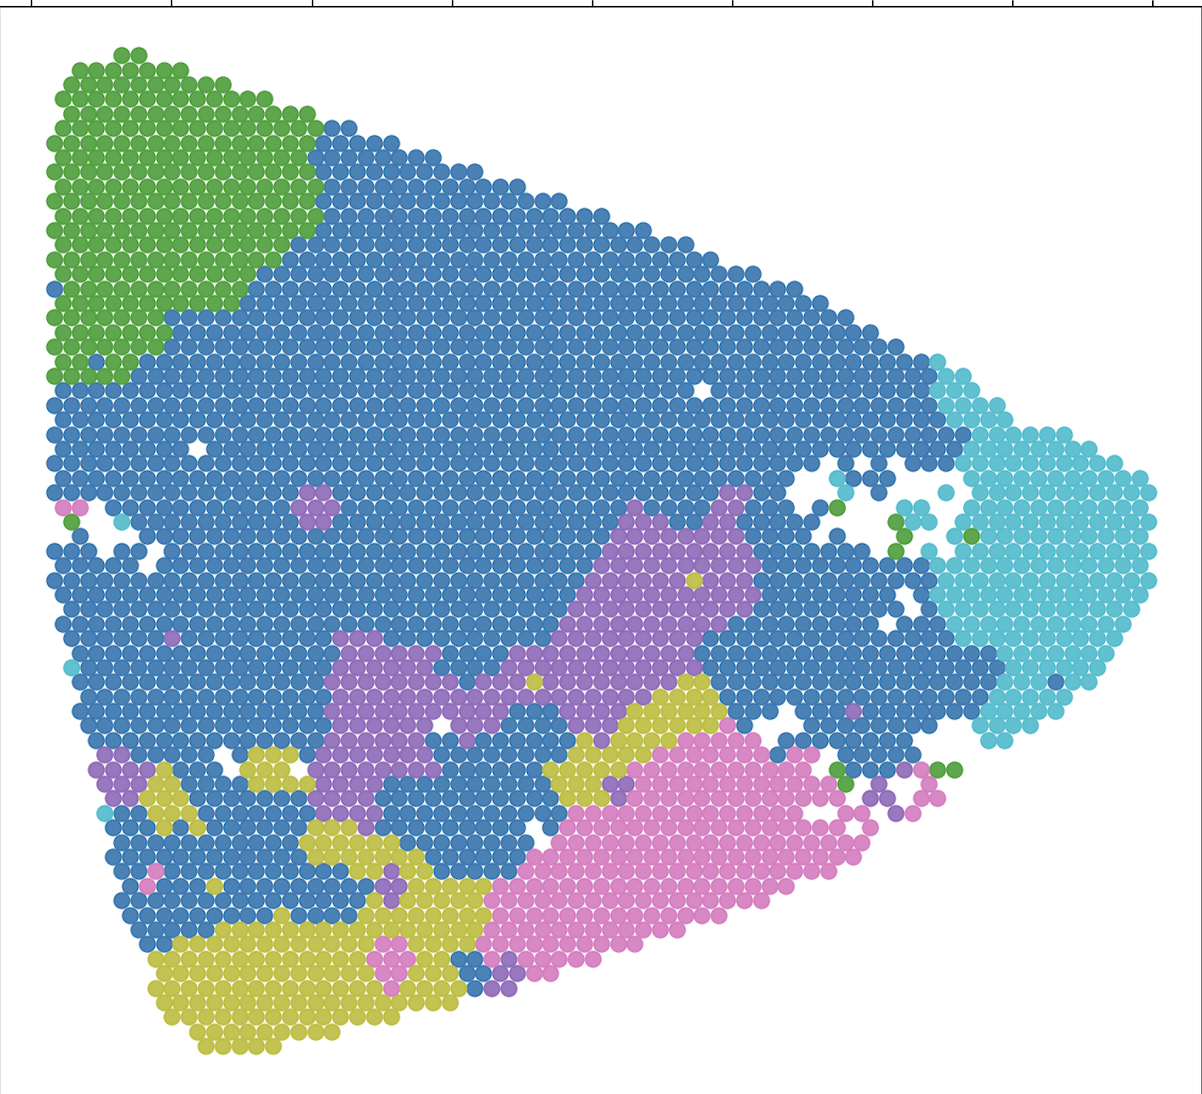
\includegraphics[width=\textwidth]{pic/anno/Y7_T_label.png}
\caption{Ground-truth annotation}
\end{subfigure}
\hfill
\begin{subfigure}[t]{0.3\textwidth}
\centering
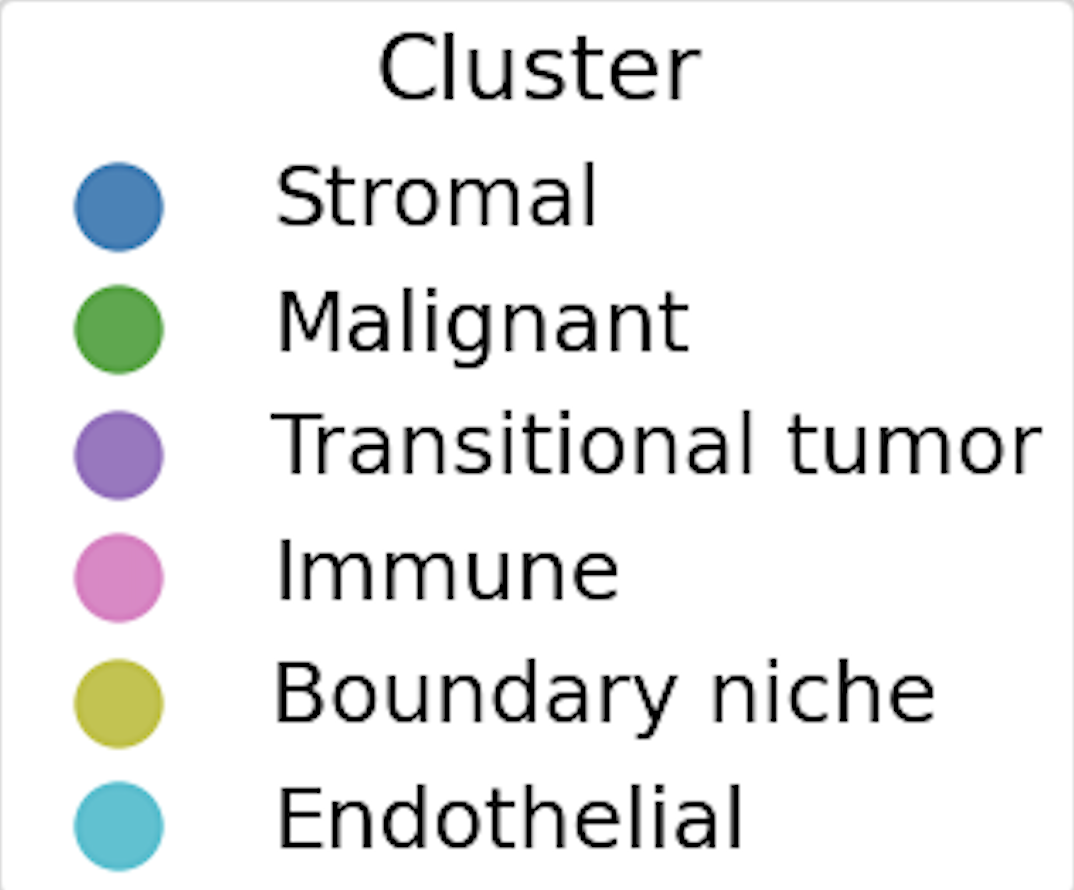
\includegraphics[width=\textwidth]{pic/anno/Y7_T_legend.png}
\caption{Region legend}
\end{subfigure}
\caption{Y7\_T ccRCC tumor slice: H\&E image and spatial domain annotations.}
\label{fig:y7t}
\end{figure}

\paragraph{Reference.} Hu, J., Wang, S.G., Hou, Y. et al. \href{https://www.nature.com/articles/s41588-024-01662-5}{Multi-omic profiling of clear cell renal cell carcinoma identifies metabolic reprogramming associated with disease progression}. \textit{Nature Genetics}, 56, 442--457, 2024.

\section{Mouse E15.5 Brain (MISAR-seq)}

This dataset profiles the embryonic day 15.5 mouse brain using MISAR-seq (Microfluidic Indexing-based Spatial ATAC and RNA-seq; Zuo et al., 2023), which simultaneously captures chromatin accessibility and gene expression. Ground-truth annotations comprise manually labeled brain regions, validated against the Allen Mouse Brain Atlas.

\begin{figure}[h]
\centering
\begin{subfigure}[t]{0.3\textwidth}
\centering
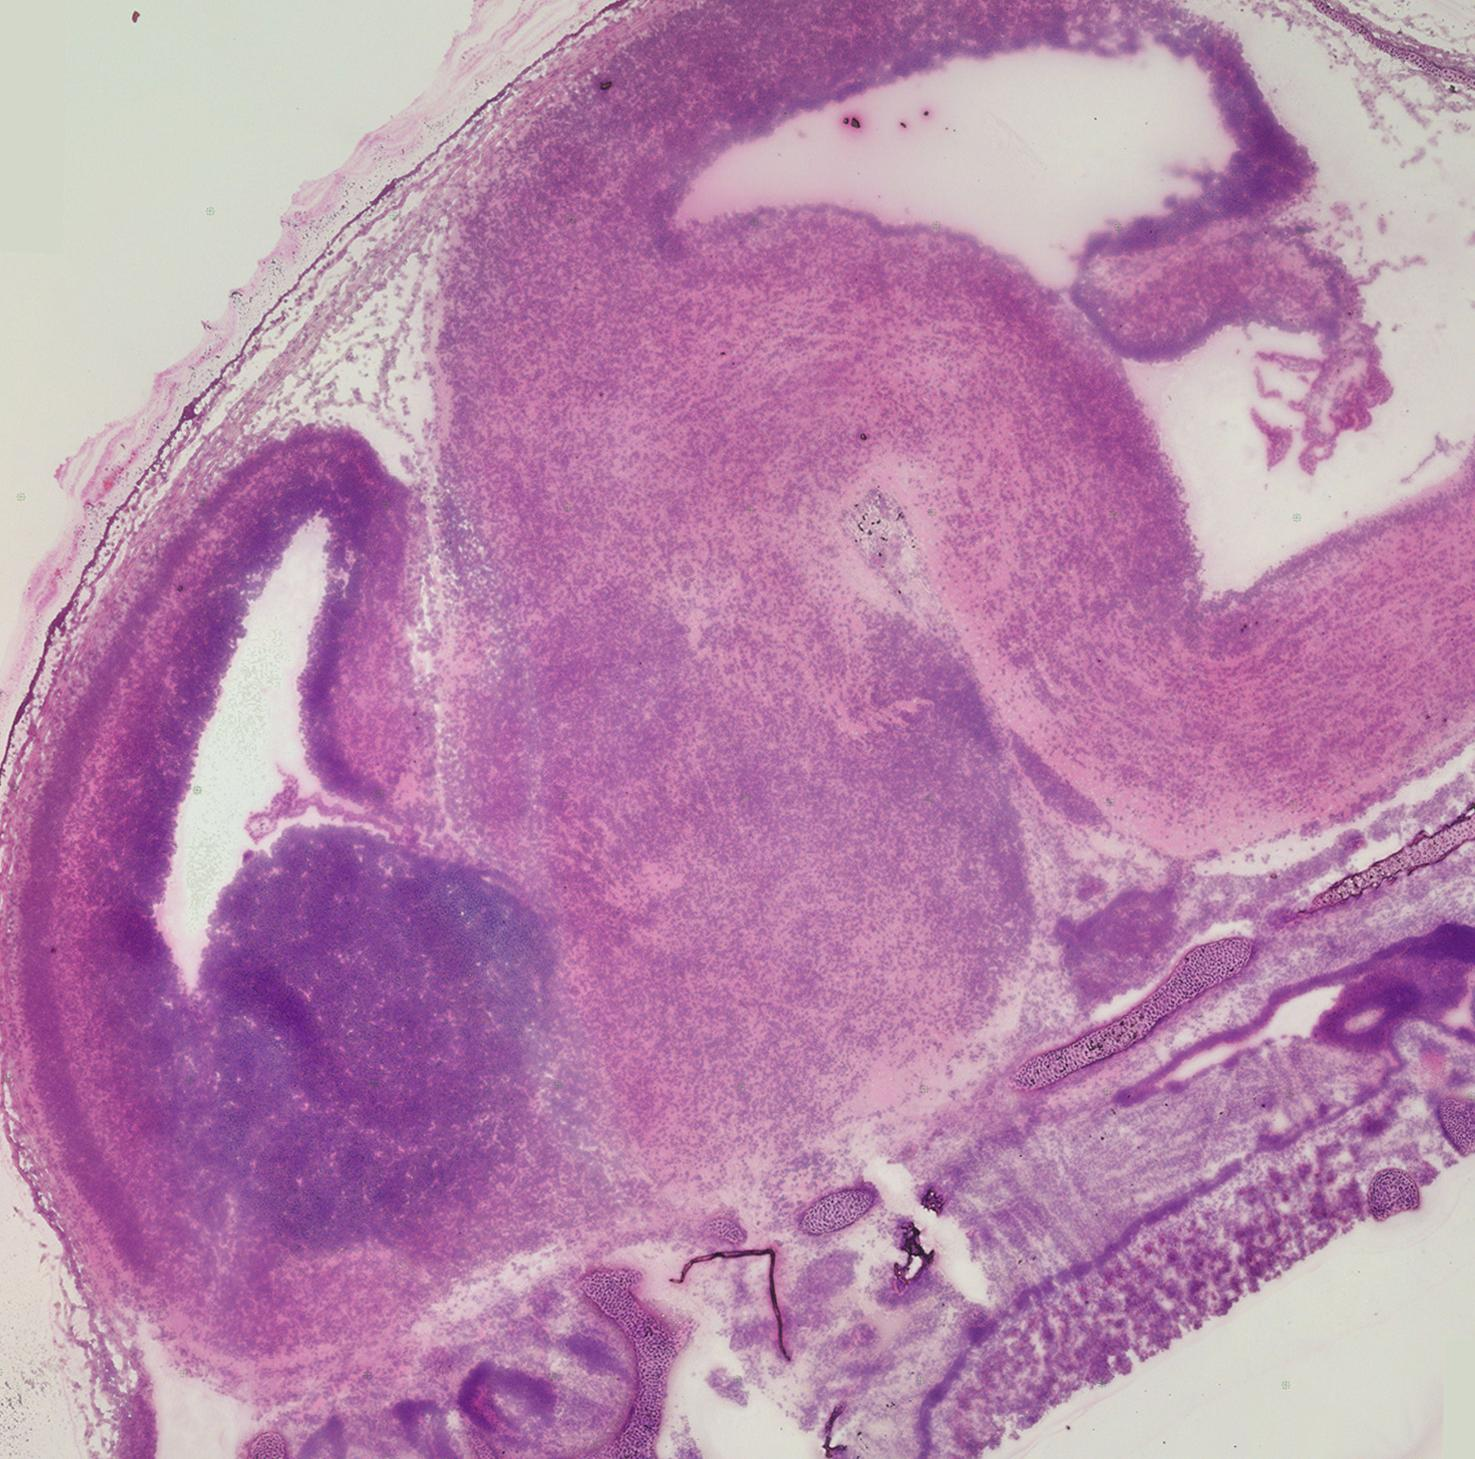
\includegraphics[width=\textwidth]{pic/he/E15_5-HE.jpg}
\caption{H\&E staining}
\end{subfigure}
\hfill
\begin{subfigure}[t]{0.3\textwidth}
\centering
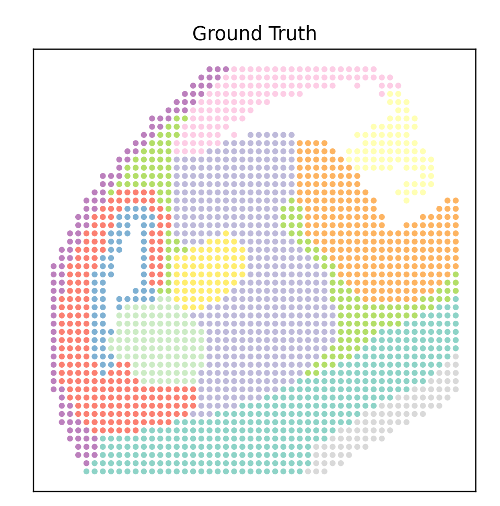
\includegraphics[width=\textwidth]{pic/anno/E15.5_label.png}
\caption{Ground-truth annotation}
\end{subfigure}
\hfill
\begin{subfigure}[t]{0.3\textwidth}
\centering
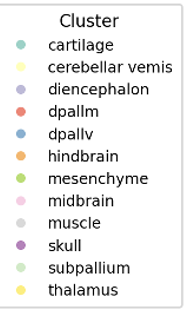
\includegraphics[width=0.6\textwidth]{pic/anno/E15.5_legend.png}
\caption{Region legend}
\end{subfigure}
\caption{Mouse E15.5 Brain: H\&E image and spatial domain annotations.}
\label{fig:e155}
\end{figure}

\paragraph{Reference.} Zuo, C., Zhang, Z. et al. \href{https://doi.org/10.1038/s41592-023-01884-1}{Simultaneous profiling of spatial gene expression and chromatin accessibility during mouse brain development}. \textit{Nature Methods}, 20(7), 1048--1057, 2023.

\section{Human Lymph Node (10x Visium CytAssist)}

Two sequential FFPE sections of human lymph node were profiled using the Visium CytAssist platform (10x Genomics; Long et al., 2024), capturing spatial gene expression (RNA) and spatial protein expression (ADT). Ground-truth annotations comprise manually labeled lymphoid compartments, annotated using high-resolution H\&E images in Loupe Browser (10x Genomics).

\begin{figure}[h]
\centering
\begin{subfigure}[t]{0.3\textwidth}
\centering
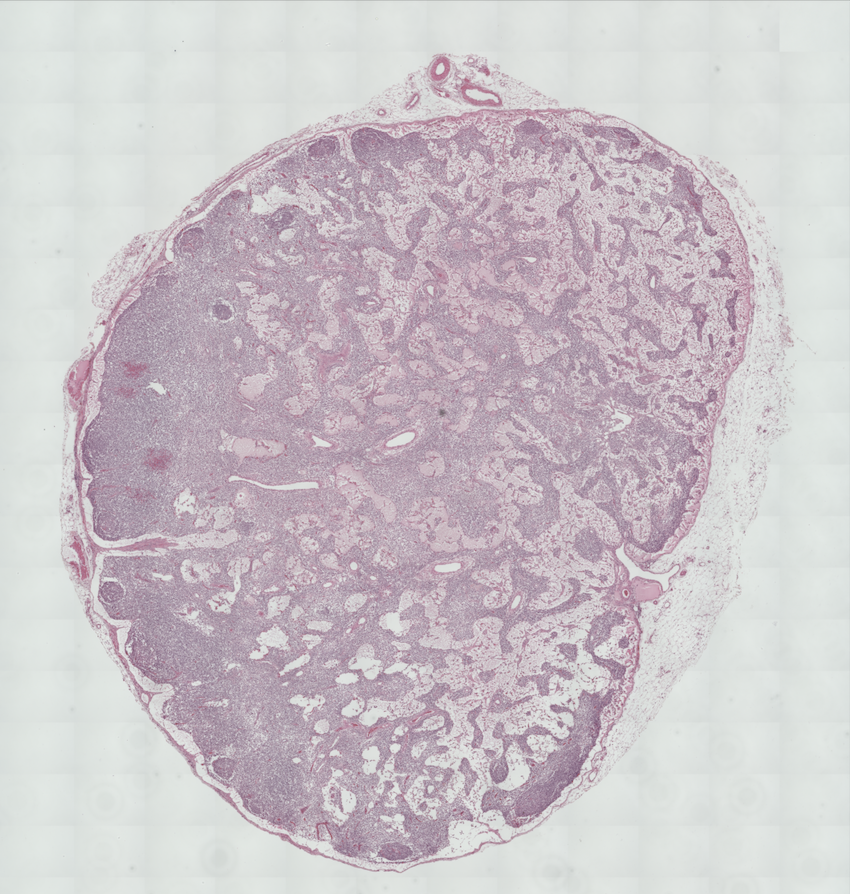
\includegraphics[width=\textwidth]{pic/he/Human_pymph.png}
\caption{H\&E staining}
\end{subfigure}
\hfill
\begin{subfigure}[t]{0.3\textwidth}
\centering
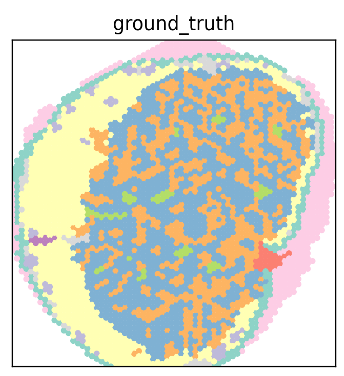
\includegraphics[width=\textwidth]{pic/anno/human_lymph_label.png}
\caption{Ground-truth annotation}
\end{subfigure}
\hfill
\begin{subfigure}[t]{0.3\textwidth}
\centering
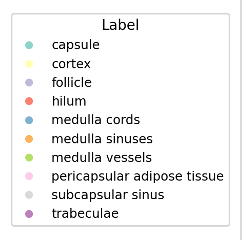
\includegraphics[width=\textwidth]{pic/anno/human_lymph_legend.png}
\caption{Region legend}
\end{subfigure}
\caption{Human Lymph Node: H\&E image and spatial domain annotations.}
\label{fig:lymph}
\end{figure}

\paragraph{Reference.} Long, Y., Ang, K.S. et al. \href{https://doi.org/10.1038/s41592-024-02316-4}{Deciphering spatial domains from spatial multi-omics with SpatialGlue}. \textit{Nature Methods}, 21(9), 1658--1667, 2024.

\section{Human Hippocampus (spatial-ATAC-RNA-seq)}

This dataset profiles an adult human brain hippocampus section using spatial-ATAC-RNA-seq (Zhang et al., 2023), which co-profiles chromatin accessibility and gene expression via deterministic barcoding in tissue (DBiT-seq).

\begin{figure}[h]
\centering
\begin{subfigure}[t]{0.3\textwidth}
\centering
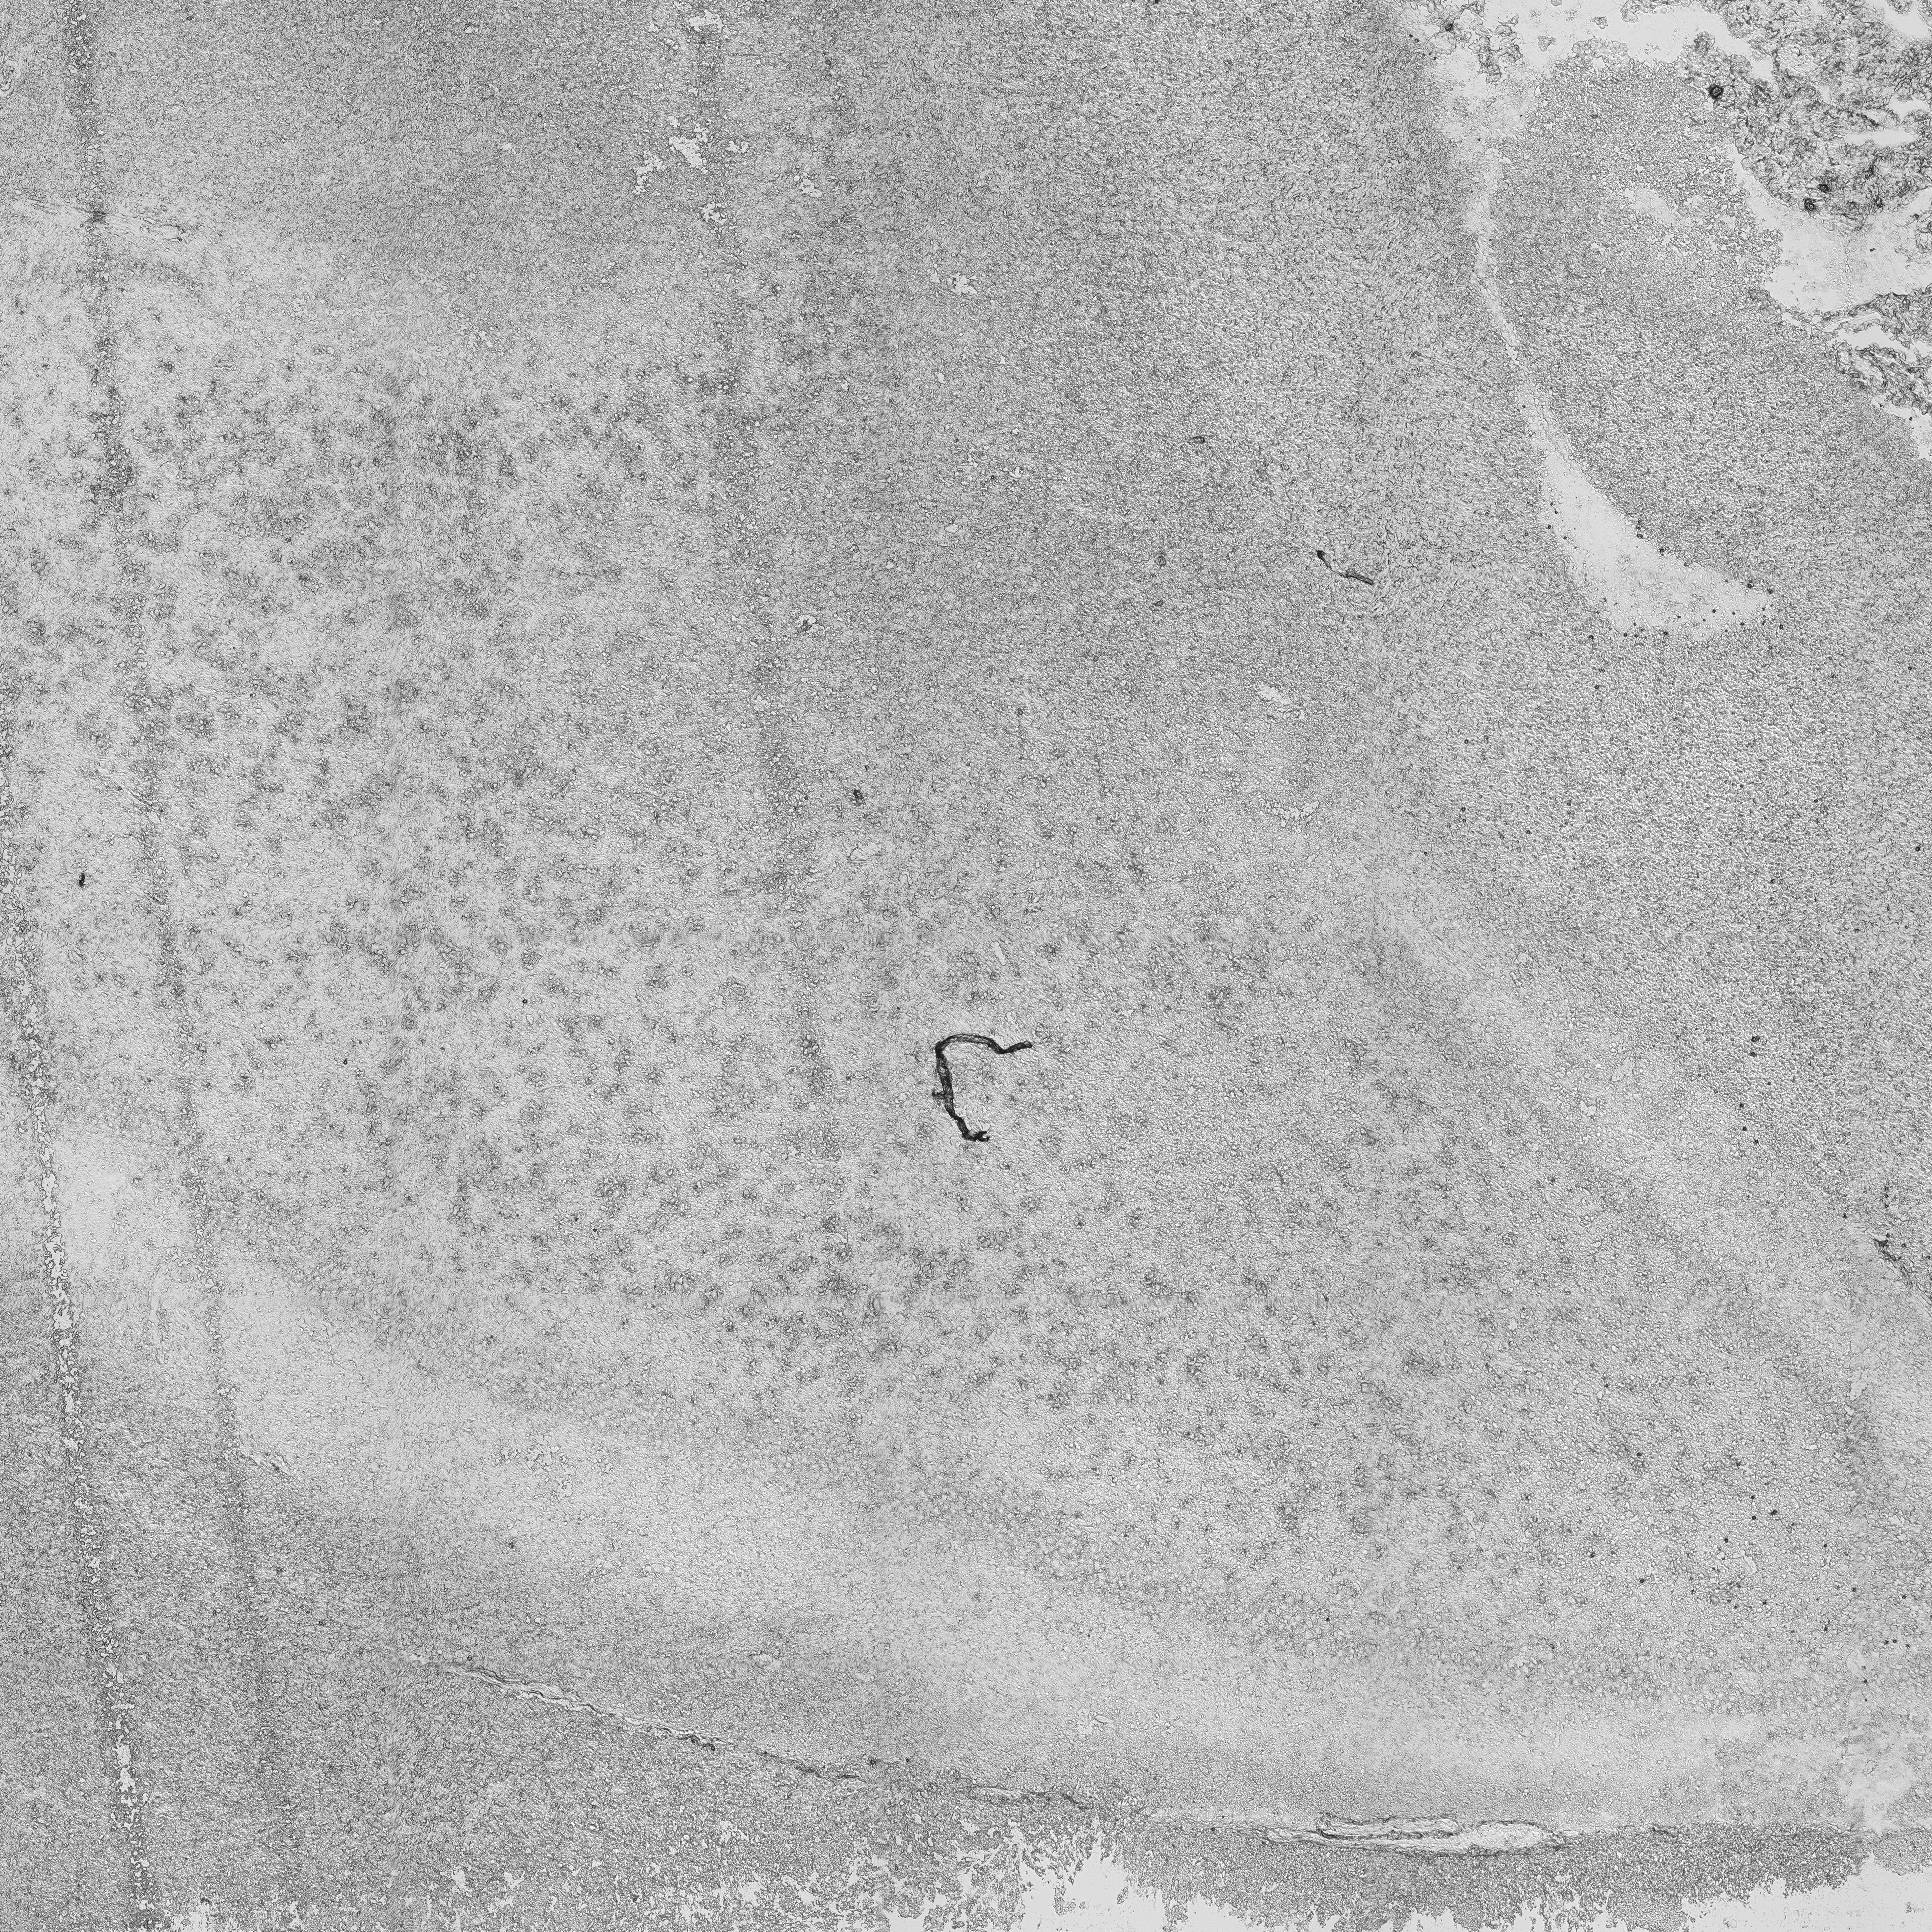
\includegraphics[width=\textwidth]{pic/he/Human_hippocampus.png}
\caption{Bright-field tissue image}
\end{subfigure}
\hfill
\begin{subfigure}[t]{0.3\textwidth}
\centering
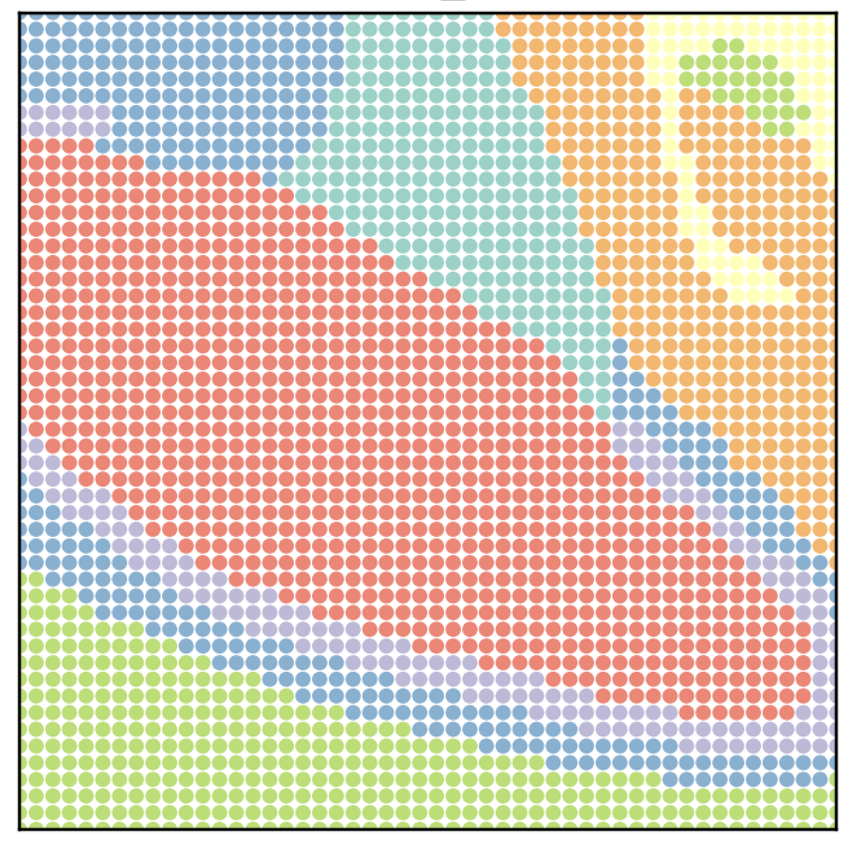
\includegraphics[width=\textwidth]{pic/anno/Human_Hippocampus_label.png}
\caption{Ground-truth annotation}
\end{subfigure}
\hfill
\begin{subfigure}[t]{0.3\textwidth}
\centering
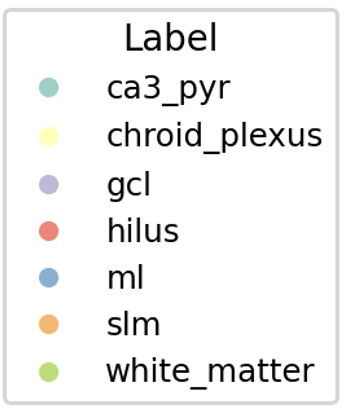
\includegraphics[width=0.6\textwidth]{pic/anno/Human_Hippocampus_legend.png}
\caption{Region legend}
\end{subfigure}
\caption{Human Hippocampus: tissue image and spatial domain annotations.}
\label{fig:hippocampus}
\end{figure}

\paragraph{Reference.} Zhang, D., Deng, Y. et al. \href{https://doi.org/10.1038/s41586-023-05795-1}{Spatial epigenome--transcriptome co-profiling of mammalian tissues}. \textit{Nature}, 616(7955), 113--122, 2023.

\end{document}
